% Slide 6: System Architecture & Workflow Pipeline
\begin{frame}
  \frametitle{Modular Pipeline Architecture}
  \framesubtitle{System Design \textbar\ Lead Presenter: Aaradhya}

  \begin{columns}[T]
    \begin{column}{0.48\textwidth}
      \begin{center}
        \IfFileExists{../report/src/images/architecture_highlevel.jpg}{%
          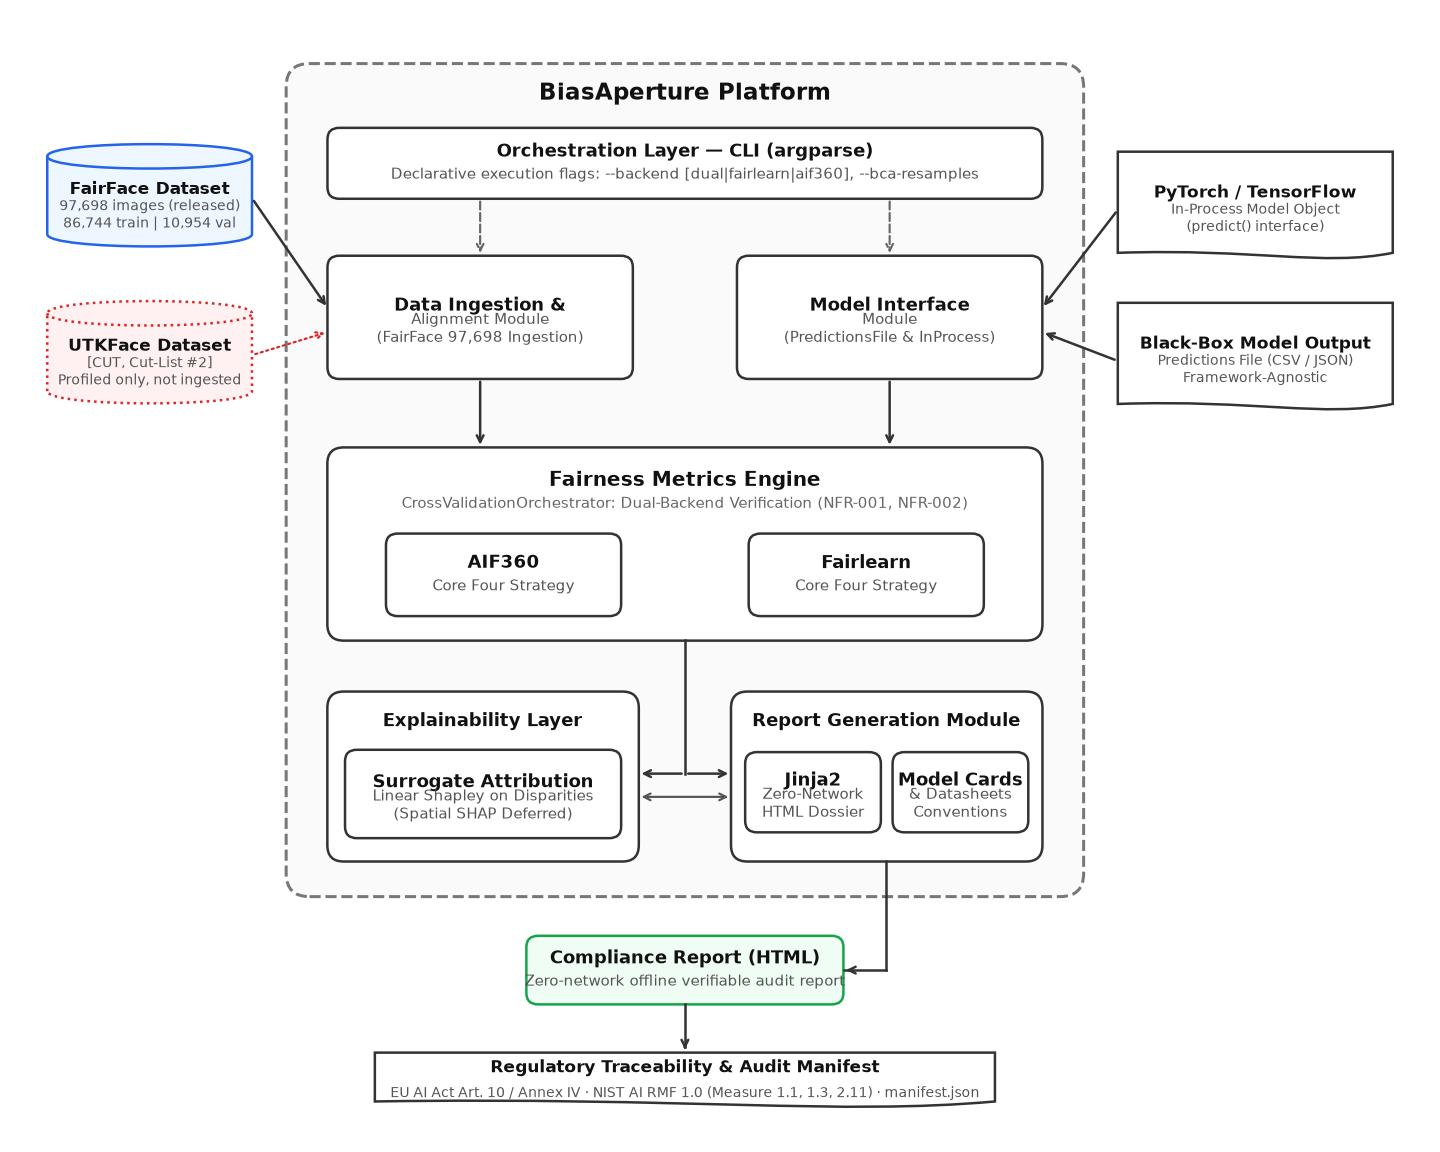
\includegraphics[width=\textwidth,height=0.52\textheight,keepaspectratio]{../report/src/images/architecture_highlevel.jpg}%
        }{%
          \begin{card}{Architecture Flow}
            Ingest $\to$ Model $\to$ Fairness Engine $\to$ Explain $\to$ Report
          \end{card}
        }
      \end{center}
    \end{column}

    \begin{column}{0.50\textwidth}
      \begin{card}{Five Cooperating Architectural Modules}
        \scriptsize
        \begin{enumerate}\scriptsize
          \item \textbf{Data Ingestion \& Alignment:} Reads FairFace; validates formats; maps labels into unified schema.
          \item \textbf{Model Interface:} Framework-agnostic prediction ingestion (CSV/JSON or PyTorch model).
          \item \textbf{Fairness Engine:} Strategy pattern over Fairlearn \& AIF360; computes Core Four metrics + stats.
          \item \textbf{Explainability Layer:} Selectively triggered proxy attribution on flagged disparities.
          \item \textbf{Report Generator:} Flat Jinja2 compiler assembling zero-network offline HTML dossier.
        \end{enumerate}
      \end{card}

      \vspace{0.1cm}
      \begin{statcard}{SOLID Design Rigor}
        \scriptsize
        \begin{itemize}\scriptsize
          \item \textbf{Single Responsibility:} Each module owns one stage.
          \item \textbf{Open/Closed (Strategy):} Adding backends/metrics requires no engine modifications.
          \item \textbf{Dependency Inversion:} Pipeline depends on abstract interfaces, never concrete vendor libraries.
        \end{itemize}
      \end{statcard}
    \end{column}
  \end{columns}
\end{frame}
